\chapter{Generación de texto al estilo de Lope de Vega: \textit{GPT}}
El codificador y el decodificador presentes en el diseño del \textit{transformer} pueden utilizarse por separado para abordar problemas en los que únicamente la entrada o la salida son una secuencia. 

Un ejemplo son los modelos generativos decodificadores, diseñados para generar una secuencia de símbolos a partir de un modelo de lenguaje aprendido y de los símbolos ya generados, que únicamente utilizan bloques de tipo decodificador. Una de las familias de modelos generativos más influyentes es GPT, nacida en 2018 con la creación de GPT-1 \cite{radford2018improving}.

En el momento de su creación, GPT-1, un modelo razonablemente sencillo basado en doce bloques de tipo decodificador encadenados, logró superar ampliamente a modelos anteriores en una variedad de tareas, como el razonamiento general o la respuestas a preguntas. Una innovación fundamental fue el uso de aprendizaje no supervisado: en lugar de depender íntegramente de bases de datos etiquetados como era habitual, GPT-1 fue entrenado de forma no supervisada sobre grandes \textit{corpus} de texto, provenientes de novelas. La red luego puede reentrenarse (\textit{finetuning}) de forma supervisada sobre conjuntos etiquetados de texto para adaptarla a tareas específicas.

Solo un año después de la publicación de GPT-1, se presentó GPT-2, un modelo con 1.5 mil millones de parámetros que demostró por primera vez de forma clara la aparición de habilidades emergentes \cite{radford2019language}. La arquitectura de GPT-2 es prácticamente una versión escalada de GPT-1 con más parámetros y mayor longitud de contexto, salvo por cambios mínimos en la inicialización de los parámetros y en la forma de normalizar las capas. Aun así, supera a GPT-1 (y a la práctica mayoría de modelos existentes en ese momento) en una varidad de tareas, incluyendo el resumen de textos, la traducción de inglés a francés, el razonamiento de sentido común o la comprensión lectora.

El \Cref{appendixA} presenta una implementación completa de la familia de modelos GPT, que puede implementarse elegantemente en unos pocos cientos de líneas.

\section{Generando texto al estilo de Lope de Vega}

\begin{figure}[tb]
    \centering
    \begin{subfigure}[b]{0.49\textwidth}
        \centering
        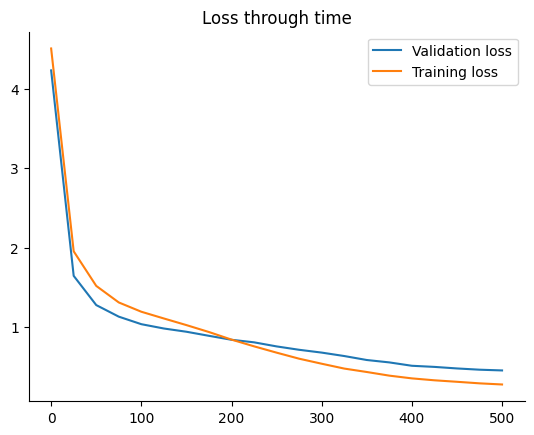
\includegraphics[width=\textwidth]{figures/chapter5/loss.png}
        \caption{Entrenamiento de GPT-1}
        \label{fig:loss}
    \end{subfigure}
    \begin{subfigure}[b]{0.49\textwidth}
        \centering
        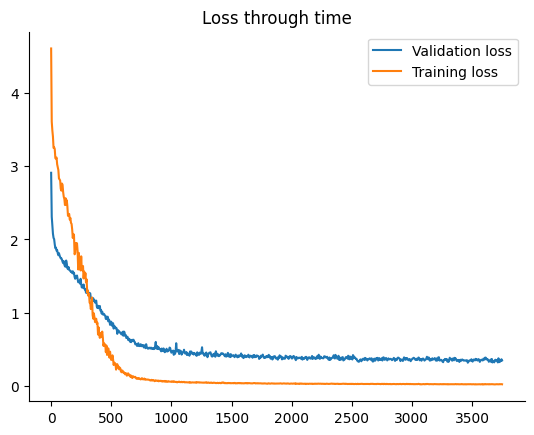
\includegraphics[width=\textwidth]{figures/chapter5/loss_big.png}
        \caption{Entrenamiento de GPT-1}
        \label{fig:loss_big}
    \end{subfigure}
    \caption{Pérdida sobre el conjunto de entrenamiento y validación a lo largo del entrenamiento.}
\end{figure}

Abordamos ahora el problema que nos hemos propuesto: entrenar la red para generar texto al estilo de Lope de Vega utilizando GPT. Con ese propósito se ha creado un conjunto de datos con alrededor de 51.000 líneas de texto plano, provenientes de distintas obras dramáticas. A fin de homogeneizar el texto y facilitar el entrenamiento se han mantenido únicamente los diálogos eliminando acotaciones, notas y textos accesorios, como los prólogos. También se han unificado los símbolos ortográficos, a fin de no ampliar el tamaño del vocabulario sin necesidad.

El conjunto de datos se ha dividido en un conjunto de entrenamiento con el \( 90\% \) de los caracteres y un conjunto de validación con el resto. Dado que no se va a evaluar el rendimiento del modelo posteriormente y el tamaño del conjunto de datos es limitado, se prescinde de un conjunto de prueba.

A fin de poder entrenar con facilidad, nos hemos decidido por un modelo de GPT muy sencillo, formado por seis bloques de tipo decodificador y con atención multicabezal con seis cabezas. Los símbolos son caracteres, representados internamente usando 384 dimensiones. La longitud de contexto es 256. El modelo tiene un total de \( 10.65 \) millones de parámetros

El modelo se ha entrenado de modo no supervisado utilizando el método de optimización \textit{Adam} (\( \epsilon = 10^{-3}, (\beta_1, \beta_2) = (0.99, 0.999) \)) durante un total de \( 5.000 \) iteraciones y eligiendo la configuración de parámetros que minimiza la verosimilitud logarítimica sobre el conjunto de validación. El modelo converge adecuadamente, como muestra la \cref{fig:loss}.

Presentamos a continuación algunas muestras del texto generado por la red. En el segundo caso, se utiliza el texto de estímulo para interactuar con la red: 

\noindent
\begin{table}[h]
  \centering
  \begin{tabular}{ ll }
    \begin{Code}
    ¿Quién es este caballero
    Que te ha enseñado a ti?
    
    SANCHO:
    Y ¿Nuño? ¿Qué importa?
    Criados son de don Tello,
    A quien me mandaste hablar:
    ¡Mal haya, amén, el consejo!
    En este valle hay diez casas,
    Y no harán llenas mis cosas
    Que te han de costar la vida.
    
    SANCHO:
    Pues ¿de qué, señor?

    NUÑO:
    Por que una puerta ha sucedido,
    En que vos su voluntad
    Y aun aomaba primero,
    \end{Code}
    & 
    \begin{Code}
    ÁLVARO:
    ¿Quién mató al comendador?
    
    COMENDADOR:
    Fuente Ovejuna lo hizo
    
    ESTEBAN:
    ¿Cómo?
    
    COMENDADOR:
    ¡Ah, señores!
    
    ESTEBAN:
    ¡A cosas tan cuerdas!

    COMENDADOR:
    ¡Perra de mi casa, ayer
    que la fe que habéis abrazar
    con la edad por ajenos!
    \end{Code}
  \end{tabular}
\end{table}

Como se puede ver, la red genera texto sintácticamente correcto y es capaz de replicar la estructura de diálogo pero la mayor parte del texto generado carece de sentido. 

Los resultados son poco sorprendentes, toda vez que estamos intentando que un modelo  muy sencillo sin ninguna noción lingüística previa ``aprenda'' castellano y lo utilice para generar una estructura correcta. 

\section{Afinando GPT-2 (\textit{finetuning})}
Los dos problemas anteriores (lo limitado del modelo y lo escaso del conjunto de entrenamiento) pueden aliviarse utilizando modelos pre-entrenados más grandes. Este modelo pre-entrenado se re-entrena o \textit{afina} (\textit{fine-tune}) sobre nuestro conjunto de entrenamiento, para adaptarlo a la tarea específica. Este segundo entrenamiento no necesita ser tan intensivo como si entrenásemos la red desde cero, pues las representaciones iniciales de la red deberían ser cercanas a las finales, lo que permite ahorrar recursos computacionales y utilizar modelos de mucho mayor tamaño.

Utilizaremos un modelo GPT-2, constituido por 12 bloques de tipo decodificador, cada uno con una atención multicabezal con 12 cabezas. La dimensión de las representación es 768 y la longitud de contexto es 1024. La división en símbolos se hace esta vez a nivel de palabra.


Partimos de una versión pre-entrenada sobre un corpus de texto de 11.5 GB, de diferentes fuentes\cite{gpt2trained} y entrenamos el modelo utilizando Adam durante 3.750 iteraciones. Como es de esperar para un modelo tan complejo entrenado sobre un conjunto tan pequeño, el modelo muestra un claro sobre-ajuste (\cref{fig:loss_big}) aunque converge adecuadamente sobre el conjunto de validación. 

Los resultados obtenidos son mucho más prometedores:

\noindent
\begin{table}[H]
  \centering
  \begin{tabular}{ ll }
  \begin{Code}
    NARV:
    Hazte santo, y verás
    Que toda la gente pasa
    De su bien y su mal,
    Y que los reyes se engañan
    Si no reparan en esto,
    Que de una palabra se vale.
    
    ARR:
    Bien dices; que éste es el fin
    De mi vida, y que adoro
    En tan dulce estado,
    Y que el fin que veo me condena,
    Darle, el fin que quiero.    

    NARV:
    Escucha, Nuño, que me pesa
    De haber venido aquí,
    Nuño, tan abatido.

    NUÑO:
    Ya del estrecho celoso,
    Hija, el corazón ensancho.

    NARV:
    ¿Qué se ha hecho el pobre Sancho,
    Que solía ser mi esposo?
  \end{Code} 
  &
  \begin{Code}
    PAD:
    ¿Por qué razon
    Donde sola mi aficion
    Puede, como la espada
    Hace al desafío burlas?
    Porque guerra y casamiento
    Es un propio pensamiento,
    Todo es guerra, y si lo es todo,
    No sales del desafío.
    Si áun hay amor, yo me rindo;
    Si el de Aragon no manda,
    Padilla, yo me rindo á mí.
    
    ÁLV:
    ¿Qué mayor contento
    Que llegar como llego?
    
    PAD:
    Aquí me deja su alteza
    Á prevenir la jornada
    Que para Granada intenta,
    Porque pienso que ha de ser
    Luégo que la primavera
    Temple la furia á los rios,
    Seque la mojada tierra.  
  \end{Code}
\end{tabular}
\end{table}

El modelo tiene limitaciones: es propenso a cambiar bruscamente el tema de conversación y el sobre-ajuste provoca que reproduzca en ocasiones oraciones enteras del conjunto de entrenamiento. En cualquier caso, se trata de resultados excelentes dado lo reducido del conjunto de entrenamiento.

Si queremos generar texto de mayor calidad, el uso de una arquitectura tan escalable como los \textit{transformers} proporciona una hoja de ruta para generar mejores predicciones: aumentar el conjunto de datos y recurrir a arquitecturas de mayor escala (teniendo en cuenta que esto puede hacer necesaria una mayor regularización).

Para hacerse una idea de los costes comutacionales implicados, afinar esta red sobre el conjunto de datos necesitó unas 10 horas en \textit{hardware} doméstico. GPT-2 no puede entrenarse de forma viable en este tipo de hardware, pues su entrenamiento necesita más de un mes en una tarjeta gráfica especializada. El afinamiento da acceso de una forma eficiente a estas arquitecturas, cuyo uso de otra manera requeriría costes inasumibles.